\documentclass[11pt]{article}
\usepackage{amsmath}
\usepackage[hidelinks]{hyperref}
\usepackage[english]{babel}
\usepackage{graphicx}
\usepackage{wrapfig}
\usepackage{subcaption}

%Gummi|065|=)
\title{\textbf{Machine learning Nanodegree\\ Capstone project}\\ Dogs vs. Cats}

\author{Richard Deurwaarder}
\date{\today}
\begin{document}

\maketitle

\section{Problem	 Definition}

\subsection{Background}
This Capstone project is about the Kaggle competition: Dogs vs. Cats Redux: Kernels Edition\footnote{\url{https://www.kaggle.com/c/dogs-vs-cats-redux-kernels-edition}}. Originally this competition ran in 2013. In the last couple of years Machine learning has changed with techniques like Deep learning becoming more popular. For this reason Kaggle reintroduced the Dogs vs. Cats competition. Comparing the results makes for a nice view into the progression of Machine learning over the last couple of years.
\subsection{Problem statement}
The competition is about determining whether an image contains a dog or a cat. A subset of the Asirra\footnote{Animal Species Image Recognition for Restricting Access} dataset is given as part of the competition. The entire dataset has over 3 million images but for this competition we're restricted to a training set of 25,000 images. For each image our model will need to provide a probability of it containing a dog, where 0 is a cat, 1 a dog, 0.5 would be unsure (this is never the correct answer for this dataset). To solve this problem I have a couple of steps to take.
\pagebreak
\subsubsection{Analysis of the dataset}
I will need to get some information about the dataset. For instance the sizes of all the images, because I need all images to be the same size. I will also look at how the luminance or brightness varies among the images.
\subsubsection{Preprocessing of the data}
Next I will preprocess the dataset. All the image sizes need to be equal, depending on the results of the data analysis I will need to adjust the size, some get padding, other might need to be cropped/rescaled. I will also normalize the images, making the luminance mean 0 and standard deviation 1. I might need to greyscale the images, this means every picture loses the color and instead all pixels will be in shades of gray. While this will make the images lose some information, it does reduce the amount of features by a factor 3. The intuition behind it is the lines, edges and other basic elements that make up the shape of the cat or dog will still be there which.
\subsubsection{Training the model}
Next up is actually making the predictions. I will use two different Convolutional neural networks for this task. The first one will use the Inception model\footnote{\url{https://github.com/tensorflow/models/tree/master/inception}}. This model is has been pre-trained on general images and you only train the part that decides what to what class an image belongs. The intuition behind this is that the pre-trained part of the network identify basic elements of images: edges, corners, areas of the same color, etc. The final part uses those basic elements to make up a category. You train that final part for your specific problem with your specific dataset, in this case dogs and cats.\\

The second model will be a similar model to the Inception model in that it uses convolution layers but it will be simpler in terms of architecture and size because all layers will be trained from scratch.
\subsubsection{Evaluating the model}
\label{evaluation-metric}
To be able to choose the best performing model, I need a metric to objectively test each model. I will use two different metrics, the first is the percentage of correctly classified images. (round the probability to nearest integer). The reason for this is to be able to compare my results with the 2013 competition. For the new competition a different metric is used, I will also test each model with this metric: 

\[
LogLoss = -\dfrac{1}{n}\sum\limits^{n}_{i=1}[y_i log(\hat{y}_i) + (1-y_i)log(1-\hat{y}_i)]
\]

The main difference, between this LogLoss function and simply a percentage of correctly classified images, is this metric punishes based on how confidently wrong a model is. So when an image is of a dog, and the predictor gives a probability of 0.1 (very confident it's a cat) this metric will give a higher loss than when the predictor would've given it a 0.4 probability, even though both would be wrong.
\pagebreak[4]
\section{Analysis}
\subsection{Data Exploration}
\begin{figure}
    \centering
    \caption{Histograms of image sizes and luminances}
    \label{fig:analysis}
    \begin{subfigure}{.5\textwidth}
  	    \caption{In pixels.}
  	    \label{fig:imagesizes}
        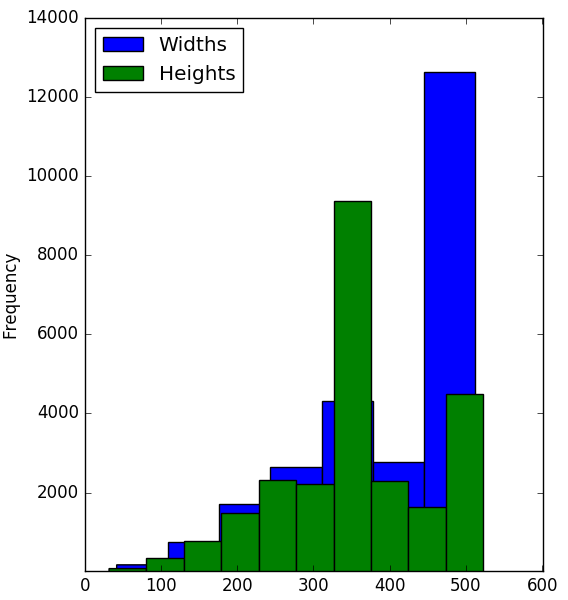
\includegraphics[width=\textwidth]{images/image_sizes}
    \end{subfigure}%
    \begin{subfigure}{.515\textwidth}
    	\caption{Mean and standard deviations.}
    	\label{fig:luminance}
    	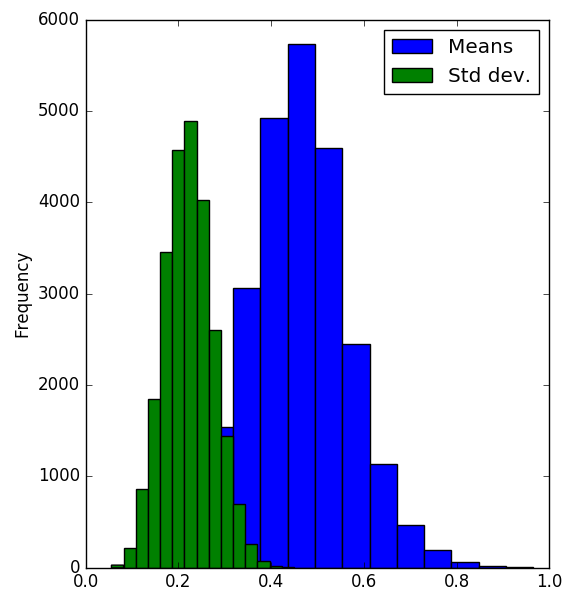
\includegraphics[width=\textwidth]{images/luminance}
    \end{subfigure}
\end{figure}
Figure \ref{fig:imagesizes} shows a lot of images have a width of just under 500 pixels. Heights are a bit more separated, a big number has a height of around 375, and at around 500 there's another peak. What the image doesn't  show is that there are a few images (less than 10) at around 1000 pixels width and/or height.\\

Looking at the luminance of each image, the average luminance of the images is around 0.45 with the standard deviations around 0.21, see figure \ref{fig:luminance}. Normalizing could be really helpful in this case.

\begin{figure}
    \centering
    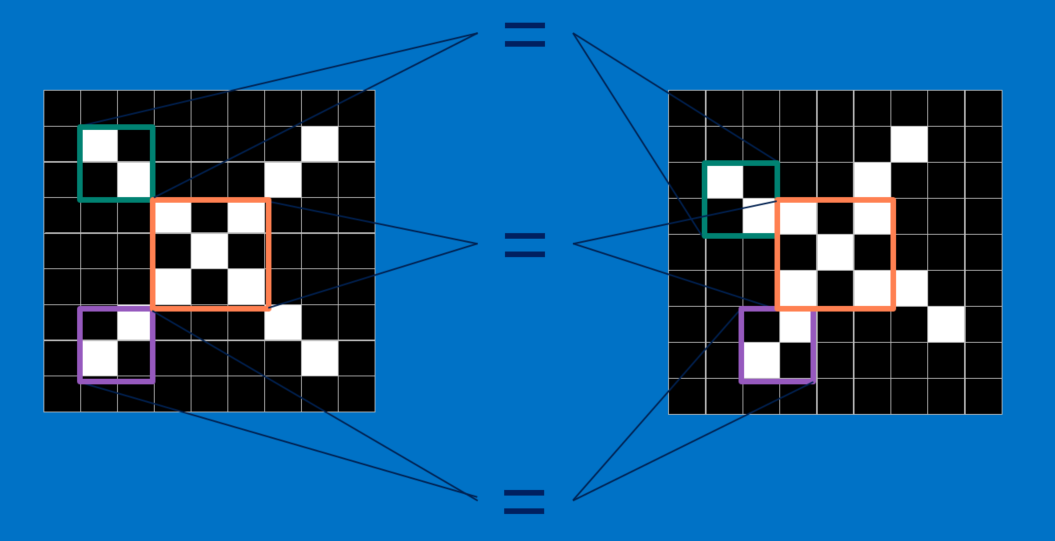
\includegraphics[width=\textwidth]{images/cnn3}
    \caption{Example of how an convolutional layer might look at an image.}
    \label{fig:cnn}
\end{figure}

\subsection{Algorithms and Techniques}
The kaggle competition specifically mentions deep learning as being one of the more promising techniques. Especially in image recognition deep learning has made some great progress. For this reason I will be using (deep) neural networks and in particular with convolutional layers to do the image recognition.\\

Convolutional neural networks for images work by looking at a small area of the image at a time. For instance a convolutional layer might look at a 2 by 2, or 3 by 3 area, and look for a cross or an diagonal line. Because the layers identify basic elements, it is also quite robust to rotation or translation of the objects it tries to identify. See figure \ref{fig:cnn}.\footnote{\url{https://brohrer.github.io/how_convolutional_neural_networks_work.html}}\\

The word `deep' in deep neural network comes from the fact that it has multiple layers stacked behind each other, making the network deeper. In this case some of those layers will be convolutional. Layers have parameters to tune, how are the weights initialized for example. Convolutional layers have even more parameters to tune, what the area will it look at (2x2, 3x3, 5x5?) What does it do with the results, max pooling, averaging? This means we have a lot of hyper-parameters to tune. 	

\subsubsection{Inception v3}
The inception model is a pre-trained model. It has been trained on a large image dataset from the ImageNet 2012 challenge, and we only have the final layer to train. This mean we don't have to tune a lot of parameters and basically have an out of the box solution. A really nice concept this model uses is the inception module. This module deals with the choice on whether to take a 1x1, 3x3 or even 5x5 area when using convolutional layers. They solve this by using all of them (1x1,3x3,5x5 and pooling layers) and letting the training algorithm choose. See figure \ref{fig:inceptionlayer}. This does take up a lot more processing power, for this reason I shall not use it in the second model.

\begin{figure}
    \centering
    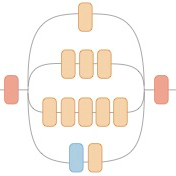
\includegraphics[width=0.25\textwidth]{images/inception-layer}
    \caption{Inception layer}
    \label{fig:inceptionlayer}
\end{figure}

\subsubsection{Building blocks of the neural network}
For my own architecture I have a lot more decisions to make, below are the building blocks I will use and what parameters I need to tune.

\paragraph{Number of layers}
I will have to decide how many of convolutional layers I will use. While more layers will allow for more complex image recognition, in general simpler models preform a lot better. Possible values I will try out are: ${4, 8, 12}$

\paragraph{Activation function}
After each layer we generally put an activation function. There are multiple choices here. Sigmoid, Tanh or Rectified linear unit (ReLU). ReLU doesn't have the gradient vanishing problem, this is because it is not limited to outputting values between $[0,1]$ but $[0,\infty]$. The gradient vanishing problem makes that the front layers train a lot slower, so on bigger networks using ReLU's can have a real advantage. Another nice property is the gradient of a ReLU function does not dissappear when it's input gets bigger.\\

Because I will be using a larger network I have chosen to use the ReLU activation function.

\paragraph{Dropout}
This is a neat and initially (for most people) counter intuitive technique. It randomly drops connections of the network while training. The idea behind it is that it causes redundancy in the network and prevent overfitting of specific patches of the input. I will try dropout layers in two parts. First in the initial input layer, secondly try out dropout layers after each convolutional layer. The weights are 0.75 and 0.5 respectively. The parameters to tune is if and where to use the dropout layers.

\paragraph{Optimizer} The optimizer will actually train the network by making small changes to the  weights of the layers. The algorithm I have chosen for this is called gradient descent. It adjusts the weights based on a loss function and a learning rate. The learning rate determines how fast the weights will change. Using a high learning rate might make the weights go into a wrong direction really fast initially and make the network unable to 'recover' and the network will not converge or have a high bias. While a low learning rate might cause the weights to change so slowly it will take forever to train.

An approach used is to make the learning rate change over time, for instance have it slowly decrease. The idea behind this is at the end of the training we only need to slightly tune the weights, and having a larger learning rate at that point might make the changes 'overshoot' the sweet spot.

Possible values I will try: 0.05, 0.1, dynamic

\paragraph{Loss function}
So the optimizer needs an loss or error function as  his will determine how the weights will change based on how wrong or correct answers are given from the network. A loss function used regulary is called Cross entropy loss.
\[
    H(p,q) = -\sum_{x}p(x)log(q(x))
\]

This is very similar to the logloss Kaggle uses (see section \ref{evaluation-metric}). In fact when $p \in \{y, 1 - y\}$ and $q \in \{\hat{y}, 1 - \hat{y}\}$ it is exactly the logloss function. 

\paragraph{Batch size}
The optimizer will run on batches of images and combine the loss of each in the batch before updating the weights. This prevents one images that is an outlier to throw off the optimizer. Sizes are generally around 16 or 32. I have chosen to use 32 images per batch.

\paragraph{Fully connected layer}
As the final layer I will use a fully connected layer, this is the layer that will decide the actual probabilities using the output of the CNN's. I will have to find out what number of nodes to use here. Possible values: ${32, 64}$



\paragraph{Softmax}
This function is used to normalize the output of the network to the [0,1] range and making the sum 1. This ends up being exactly the answer we want our network to give because we're interested in the probabilities of an image being a cat or dog.

\paragraph{Epochs}
This is the final variable, this decides how many times the training algorithm will loop over the data, on larger networks with small learning rates might be needed to adjust the weight accordingly. Possible values [1,10].
\subsection{Benchmark}
There are two sources of results to which I can test my two models. From the 2013 competition and the 2016 competition. These use different kind of metrics which cannot be converted to one or the other, so I'll compare both of them. Table \ref{leaderboard2013} shows the top 5 results and the 25th and 50th percentile of both competitions. The 2013 competition has scores ranging from 0.98 to 0.99, which will be a tough score to beat. The third column shows the 2016 scores. These scores have been accumulated from 2 September 2016 to 5 January 2017. While the competition is still ongoing, it does provide for a good baseline.

\subsubsection{Hyperparameter search}

\begin{tabular}{|l | l|}
	\hline
	Parameter & Values\\
	\hline
	Number of layers & 4, 8, 12\\
	Connected layer nodes & 32, 64\\
	Dropout on input & False, 0.75\\
	Dropout on hidden layers & False, 0.5\\
	Learning rate & 0.05, 0.1, dynamic \\
	Epochs & 1, 10\\
	\hline
\end{tabular}
\label{hypersearch}


\begin{table}
\centering
\begin{tabular}{l | ll}
	\# & Score 2013 & Score 2016\\
	\hline
	1 & 0.04220 & 0.03883\\
	2 & 0.98309 & 0.04097\\
	3 & 0.98171 & 0.04135\\
	4 & 0.98171 & 0.04162\\
	5 & 0.98137 & 0.04219\\
	\hline
	25th & 0.95726 & 0.10264\\
	50th & 0.73006& 0.24157
\end{tabular}
\caption{Leaderboard for the Kaggle Dogs vs. Cats competition of 2013 and 2016. The 2013 scores are in percentage correctly classified, higher is better. The 2016 scores in LogLoss, lower is better.}
\label{leaderboard2013}
\end{table}

\section{Methodology}
\subsection{Data preprocessing}
I have chosen use a final image size of 500x500. I choose larger values rather than values which have the biggest frequency, this is because when padding an image with grey pixels. I don't lose any information in the image. When having to make them smaller I need to scale them and thus lose some information which I would like to minimize. Because 500x500 is a rather large size to work with I have also chosen to convert all the images to grey scale images to reduce the amount of memory needed.\\
All images have had their luminance normalized to make sure all features/pixels are on the same scale.

\subsection{Implementation}
\subsubsection{Hardware}
A problem I initually run into was memory issues. I assumed this happened because of the larger size of the images I work. After giving it some tries with 128x128 images it worked a lot better. However because it did seem to hurt the results I went back to 500x500 but used grey scale images and ran the code on AWS\footnote{Amazon Web Services} to provide more memory and computing power to train and test the networks, this also greatly sped up the training times which made it a lot easier to play around with code and see how different configurations impacted the results.

\subsubsection{Train, validation, test dataset}
Kaggle provides a training and test set. However because it is an competition their test set does not have any labels, this means we only get the logloss after submitting the answers for their test set to Kaggle website. Thus we can not easily use their test set to evaluate different versions of the model.\\

For this reason I have decided to split the training set up into an new training and test set. This split is used for all models. Each model will randomly pick a new validation set from this smaller training set whenever needed.

\subsubsection{Inception model}
Using the inception v3 model of google the implementation was straight forward, using the documentation page\footnote{\url{https://github.com/tensorflow/models/tree/master/inception}} it was a matter of compiling the library, sorting the images in the correct directories (one directory per class), training and running the model. After the training I had to run it on the test set and calculate the accuracy and logloss.

\subsubsection{Custom model}
The custom model is build using Tensorflow via it's Python API. Initially I wanted to build it using the inception modules as used in the inception model. However because this increases the amount of weights needed to change by such a great amount I took too much time and data than I had available for the network to converge. For this reason I switched by to single convolutional layers.\\

Even after having switched to single conv layers I ran into memory problems. I had to load the validation set one at the time, because it was too large to send it to the GPU memory whole.\\

Apart the refinement above, actually building the classifiers was quite straight forward using Tensorflow. Because I knew I would have to test to several models I've made sure each hyperparameter was easily adjustable. While training the classifier I keep track on how well the classifier does on the train and validation set. At the end of the training I test it on the test set to be able to compare with other versions. All data points are saved in csv files so I'm able to plot and verify if at some point I start overfitting or if an combination of parameters doesn't work at all.

\section{Result}
\subsection{Model Evaluation and validation}
\subsubsection{Inception model}
The inception model handles all the validation and testing within the provides scripts. Simple by providing the percentages of the training set used for the validation set gave me following results. For the testset a logloss of 0.027707 and an accuracy of 99.4\%.
\subsubsection{Custom model}
I tested 144 different models for all the combinations of the hyperparameters (See table \ref{hypersearch}). I picked the top 5\% results and looked at the frequencies of the chosen parameters. These were the results (bold indicates the highest frequency):

\begin{tabular}{ c | c | l}
 Category & Parameter & Frequency\\
 \hline
                  & 4 & 1\\
 Number of layers & \textbf{8} & \textbf{4}\\
                  & 12 & 2\\
 \hline
 Connected layer nodes & \textbf{32} & \textbf{7}\\
                       & 64 & 0\\
 \hline
 Dropout on input & \textbf{False} & \textbf{7}\\
 & 0.75 & 0\\
 \hline
 Dropout on hidden layers & \textbf{False} & \textbf{5}\\
 & 0.5 & 2\\
 \hline
 & \textbf{0.05} & \textbf{3}\\
 Learning rate & 0.1 & 1 \\
 & dynamic & 3\\
 \hline
 Epochs & 1 & 2\\
 & \textbf{10} & \textbf{5}\\
 \hline
\end{tabular}

\paragraph{} The learning rate has a tie between 0.05 and dynamic, I've chosen to go for the 0.05 because it has a lower complexity which is generally better for a model. Thus the best performing classifiers have these properties in common:\\

\begin{tabular}{|l | l|}
	\hline
	Parameter & Value\\
	\hline
	Number of layers & 8\\
	Connected layer nodes & 32\\
	Dropout on input & False\\
	Dropout on hidden layers & False\\
	Learning rate & 0.05\\
	Epochs & 1, 10\\
	\hline
\end{tabular}

\paragraph{} Although I have actually tested this model (in my exhaustive search i tested all variants), it's not clear whether it was done training yet. To verify this I plotted the LogLoss of the training set versus the LogLoss of the validation set. I reran the classifier, but used a bigger epoch of 50 (this results in around 27000 steps) to see where it would finish training and start overfitting or memorizing the data. Figure \ref{fig:overfitting} shows pretty erratic loglosses in the validation data but it does show a trend of LogLoss going down gradually up to the 5000 steps. After that point the train and validation loglosses start to seperate from each other indicating the model it's overfitting on the training data after that point.

\paragraph{} After training the model once more but stopping after 5000 steps (9 epochs). The logloss of the test set was 0.241 with an accuracy of 76.12\%.

\begin{figure}
    \centering
    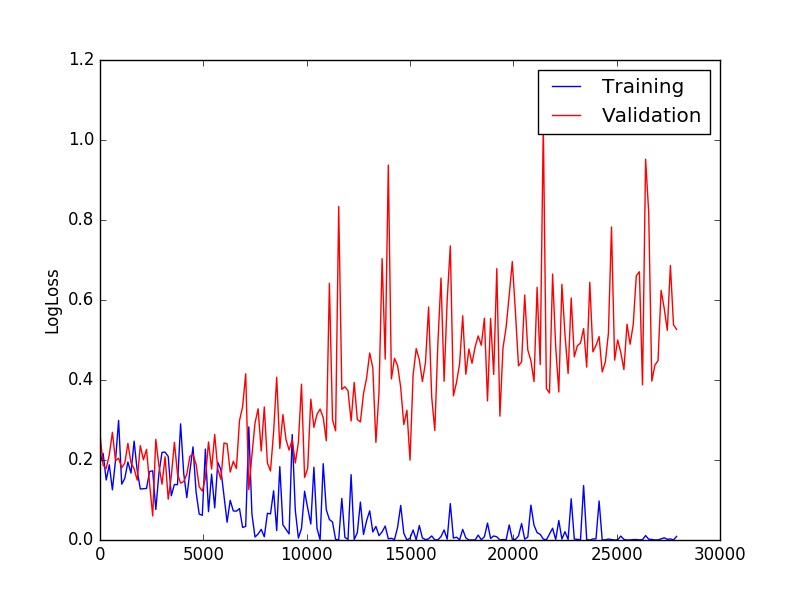
\includegraphics[width=0.75\textwidth]{images/overfitting}
    \caption{Overfitting}
    \label{fig:overfitting}
\end{figure}

\subsection{Justification}
The inception model is clearly the better performing model. I've used this model to create an actual submission to compare the model with the other participants of the competition. It achieved a score of 0.04994, which brings it to the 21th position, or top 5\%. Which is pretty good.
Comparing the model to the 2013 competition is a bit trickier, because it doesn't allow new submissions. But the top score on that competition had a 98.9\% accuracy, while the inception model had a 99.4\% accuracy on it's own test set. Although I cannot entirely test it, it does seem to outperform all the models in the 2013 competition which is really good.
\section{Conclusion}
\subsection{Reflection \& improvements}
I've provided two different approaches to the problem. With the inception model out performing the custom model.  
The hardest part was finding a good architecture for the custom model, while keeping the time to train low. Further improvements could be found here. In particular allowing for a lot more training time. Retraining the inception model only takes 15 to 30 minutes, but the first layers have been trained for a long time and we can utilize that training time without too much cost. My custom model does not have this advantage. Introducting a more complex architecture with possibly inception modules and training on a bigger dataset would surely provide with more promising results.

\end{document}
